% -----------------------------------------------------------------------------
%                                 Background
% -----------------------------------------------------------------------------
\newpage                                                   \chapter{Background}


%------------------------------------------------------------------------------
\section{                  Sound Localization                                 }


Sound localization refers to a listener's ability to identify the origin of a
detected sound in both direction and distance.  Mammalian sound localization
mechanisms have been extensively studied. The following section provides the
reader with background information necessary for the remainder of the work.

\begin{figure}[htbp]
\centering
  \begin{minipage}[b]{.6\linewidth}
    \centering
  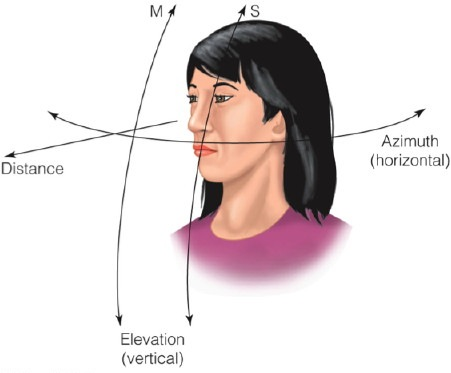
\includegraphics[width=1\linewidth]{images/binaural_reference.jpg}
    \caption{Measurements used for spatial sound processing analysis.}
    \label{fig:binaural_measurements}
  \end{minipage}
\end{figure}


The brain is able to utilize subtle differences in a sound's intensities,
spectral and timing cues to locate the origin of a given sound source.  Often
the measurements used to place a sound relative to a subject are the
\textit{azimuth} (the horizontal angle), the \textit{elevation} (the vertical
angle) and the \textit{distance} (for static sounds) or \textit{velocity} (for
sounds that are moving) ~\cite{shannan2010audiology}.  These measurements are
illustrated in figure ~\ref{fig:binaural_measurements}.  Also portrayed in this
illustration  are two vertical axis: \textit{M} refers to the axis aligned to
the median of the subject and \textit{S} refers to the vertical axis aligned to
a side parallel with the subject's ear.

The primary mechanisms that an auditory system uses to determine a sound's
location including time and level differences between the signals arrival at
each of the subject's ears  are illustrated below:

\textit{Interaural Time Difference} (ITD) is shown in figure
~\ref{fig:binaural_time_difference}. The figure illustrates how sound emitted
from different sources reach both ears. The sound emitted from point (A) which
is directly in front of the subject arrives at both ears at the same time.
However, when the tone is off to the side (B), it reaches the listener's right ear
before it reaches the left. Interaural time differences is precisely the time
difference that the ears perceive the same sound.  ITD applies to low frequency
localization for sounds that are less than approximately 1500Hz.  The average
distance between human ears is 20 cm resulting in a 600 microsecond delay between
the incident sound in one ear and hearing in the other for a sound emitted from
point A.  As the azimuth changes, the delays increase, and provide a feature
that the brain can use to place sound.


\begin{figure}[htbp2]
  \begin{minipage}[b]{.45\linewidth}
    \centering
    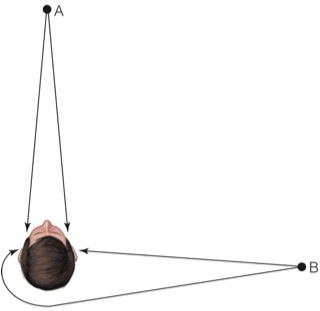
\includegraphics[width=.8\linewidth]{images/binaural_interaural.jpg}
    \caption{Diagramed interaural time differences.}
    \label{fig:binaural_time_difference}
  \end{minipage}
  \hspace{0.5cm}
  \begin{minipage}[b]{0.5\linewidth}
    \centering
  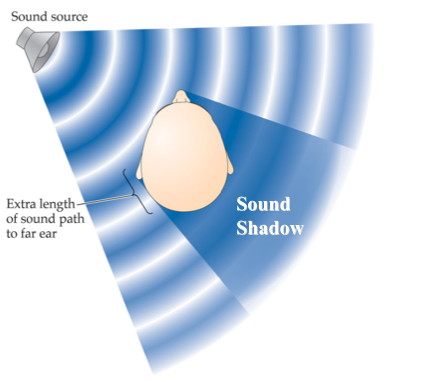
\includegraphics[width=.9\linewidth]{images/binaural_level.jpg}
    \caption{Diagram of sound level differences.}
    \label{fig:binaural_sound_level}
  \end{minipage}
\end{figure}


\textit{Interaural Intensity Delay} (IID), like ITD is also dependent on the
frequency of the sound emitted.  If a sounds wavelength is equal to or greater
than the listener's head then the sound will diffract around the head and be
heard with the same intensity as the incident wave.  What is being displayed in
figure ~\ref{fig:binaural_sound_level} is a high frequency sound where
absorption of the sound energy occurs by a solid medium (in this case, the
subject's head). This absorption of sound energy is called a sound shadow
because there is effectively zero sound energy from the original source in that
space. The  difference in magnitude of the frequency perceived by both ears is
what is  measured by interaural intensity delays.


%------------------------------------------------------------------------------
\section{                  Binaural Audio                                     }

\textbf{binaural audio} is simply audio that is engineered with the intention
of creating a 3-D stereo sound sensation for a listener.  The goal is often to
simulate the listener's actual presence in a virtual environment where the
recording was actually made. This acoustic virtualization can be accomplished
with the use of specialized hardware or signal processing techniques.

The only requirement to produce three dimensional audio systems or to render
sound images around a listener is stereo sound output from either headphones
or loud speakers~\cite{thackara2005bubble}. In the case of 3D audio systems
that use headphones, the 3D audio cues to localize a virtual source can be
perfectly reproduced at the listener’s eardrums because the headphones isolate
the listener from external sounds and room reverberations.

\textbf{Transaural audio} is the name for the technique of delivering signals to
the ears of a listener using stereo loudspeakers. The primary difference between
this technique and binaural audio is that transaural filters must take into
account room reverberations.  Transaural audio filters a binaural signal such
that the subject can process the subsequent stereo representation as a 3D signal
given the reverberations of the listener's environment.  This technique was
first put into practice by Shroeder and Atal ~\cite{ schroeder1963computer,
schroeder1970digital }. It is possible to produce the accuracy of binaural audio
from headphones through the use of loudspeakers, as is often observed with high
end sound systems. Systems capable of calibrating the audio to a moving user
with stationary stereo speakers in an open  environment with the aid of head
tracking web cams have been demonstrated. Researchers have shown how both the
audio transformations necessary to mimic the physics of the 3D sound waves and
the placement of the virtual sound sources relative to the listener can be
updated in real-time using only loudspeakers~\cite{song2010personal}.

Ultimately, both binaural audio and transaural audio systems aim  to perfectly
calibrate sound placement to create an experience that provides the user with
the perception that sound is placed in a 3D environment that exists around them.



%------------------------------------------------------------------------------
\subsection{                 Binaural Solutions                               }

Binaural audio has a history dating back to 1881 where an array of microphones
were installed on the front edge of the Opera Garnier allowing telephone
subscribers to enjoy the music through their telephones with specialized
headsets~\cite{jost2000transaural}.  Since then, the novelty of the technology
has waxed and waned with the introduction of the radio, television, and personal
walkmans.  Binaural audio is experiencing a resurgence in popularity,
specifically within the audiophile communities as headphones have become
cheaper and capable of producing higher quality audio.


\begin{figure}[htbp3]
  \begin{minipage}[b]{.45\linewidth}
    \centering
    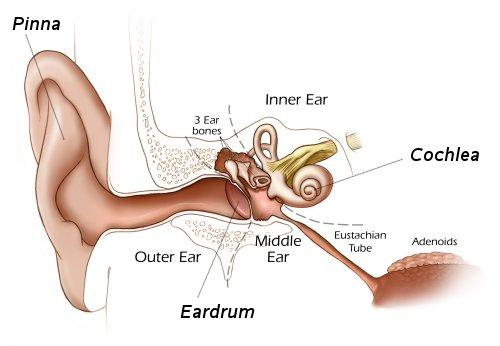
\includegraphics[width=1\textwidth]{images/ear_diagram.jpg}
    \caption{Anatomy of the ear.}
    \label{fig:ear_diagram}
  \end{minipage}
  \hspace{0.5cm}
  \begin{minipage}[b]{0.5\linewidth}
    \centering
    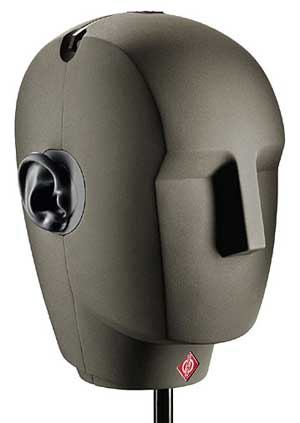
\includegraphics[width=.4\textwidth]{images/binaural_mic.jpg}
    \caption{Binaural microphone with the exact dimension and density as a human
     head. There are two input channels corresponding exactly to the location of
     human eardrums.}
    \label{fig:binaural_mic}
  \end{minipage}
\end{figure}

There are primarily two ways to produce binaural audio.  The audio can either be
generated using signal transformations or recorded.  Figure
~\ref{fig:binaural_mic} is a binaural microphone where two high-fidelity
microphones are mounted inside a dummy head inset in ear shaped molds allowing
the system to fully capture all of the audio frequency adjustments that happen
naturally as sound is warped by the human head. There exist many variations of
the microphone, each targeting different types of output (e.g. playback on
headphones versus loud speakers).


The second method to produce binaural audio is through the actual manipulation
of two sound channels using a \textbf{Head Related Transfer Function} (HRTF).
The general idea is to reproduce the acoustic transformations that would
normally occur at the listener's ears in a natural listening situation.
Specifically, the HRTF describes exactly how a given sound wave input,
originating from some location and having some frequency, is filtered by the
diffraction and reflection properties of the head, pinna, and torso before the
sound reaches the mechanical parts of the eardrum and inner ear (figure
~\ref{fig:ear_diagram}).


This process is accomplished by convolving each source signal with a pair of
HRTFs corresponding to the sound sources intended location.  The resulting
signal is presented to the user through headphones. Figure
~\ref{fig:binaural_spatializer} demonstrates the spatialization of a single
sound source from an arbitrary distance and azimuth.  The direction of the
source ($\theta$ = azimuth,  $\phi$ = elevation) determines which pair of HRTFs
to use and the distance (\textit{r}) determines the gain.  Figure
~\ref{fig:binaural_spatializers} demonstrates how to spatialize multiple sound
sources with constant level reverberation to enhance the listener's perception
of distance ~\cite{gardner1995transaural}.

\begin{figure}[htbp4]
  \begin{minipage}[b]{.45\linewidth}
    \centering
    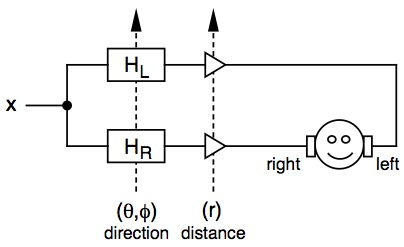
\includegraphics[width=.8\linewidth]{images/binaural_spatializer.jpg}
    \caption{Single source bianaural spatializer}
    \label{fig:binaural_spatializer}
  \end{minipage}
  \hspace{0.5cm}
  \begin{minipage}[b]{0.5\linewidth}
    \centering
  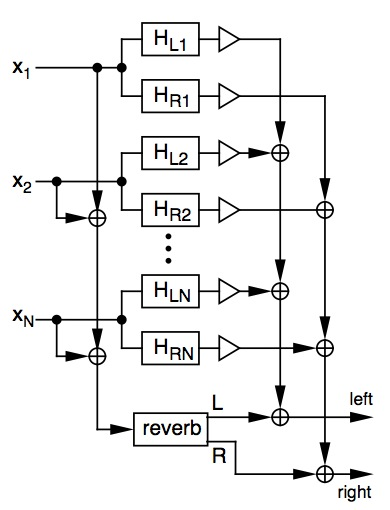
\includegraphics[width=.5\linewidth]{images/binaural_spatializers.jpg}
    \caption{Multiple source binaural spatializer.}
    \label{fig:binaural_spatializers}
  \end{minipage}
\end{figure}




%-----------------------------------------------------------------------------%
\subsection{                  Binaural Issues                                 }

Given that humans are capable of processing sound signals to place the audio
source in space, either prerecorded or simulated sounds used to produce the
auditory experience of one or more sound sources arbitrarily located around a
listener are subject to certain constraints. Once recorded or produced, the
spatialization requires stereo playback. To accurately reproduce the effect of
hearing a sound in person, given the location of objects, user specific HRTFs
should be calibrated to the individual user. In practice, average HRTFs work
well enough for most young adults~\cite{wenzel1993localization}. Secondly, the
concept of externalization which is the placement of the sound sources in the 3D
plane suffers when users use in-ear headphones.  What can occur with in ear
headphones is that the 3D plane is perceived to be inside of the head (a process
called internalization). Other minor issues include the variance between
individual user's in their ability to perceive sound elevations.


%-----------------------------------------------------------------------------%
\subsection{                  Accessibility                                   }

There are many existing solutions that enable blind users to access computer
interfaces.  Screen readers such as JAWS and Windows-Eyes are proprietary special
purpose software solutions that cost more than \$1000 per installation. Free
alternative solutions do exist, such as NVDA, Orca and the Linux Screen Reader
available to users on Linux and Windows~\cite{bigham2008webanywhere}.  The
Macintosh operating system comes standard with Voice Over and is available on
all Macintosh computers and iOS devices. There are other solutions available for
web content and browsers as  well as custom hardware solutions aimed at
providing accessibility solutions. But these products that provide accessible
solutions only produce monaural audio and provide no audio localization.
